\documentclass[12pt,a4paper,twoside,openright]{book}

%===========================================================
% ===================== FONTS & TYPOGRAPHY =================
%===========================================================
\usepackage{fontspec} % Requires XeLaTeX or LuaLaTeX
\setmainfont{Libertinus Serif}[
  BoldFont={Libertinus Serif Bold},
  ItalicFont={Libertinus Serif Italic},
  BoldItalicFont={Libertinus Serif Bold Italic}
]
\setsansfont{Libertinus Sans}
\setmonofont{Fira Code} % For code snippets

\usepackage{microtype} % Better typography
\usepackage{setspace}
\onehalfspacing

%===========================================================
% ===================== PAGE LAYOUT ========================
%===========================================================
\usepackage[a4paper,inner=35mm,outer=25mm,top=30mm,bottom=30mm,headheight=16pt,headsep=12pt,footskip=18mm]{geometry}
\linespread{1.15}

%===========================================================
% ===================== COLORS =============================
%===========================================================
\usepackage{xcolor}
\definecolor{myblue}{RGB}{0,65,135}
\definecolor{chaptergray}{gray}{0.13}

%===========================================================
% ===================== CHAPTERS & SECTIONS ===============
%===========================================================
\usepackage{titlesec}
\usepackage[Bjornstrup]{fncychap} % Modern chapter style
\ChTitleVar{\Huge\bfseries\color{myblue}}
\ChRuleWidth{1pt}

\titleformat{\section}
  {\Large\bfseries\headingfont\color{myblue}}
  {\thesection}{1em}{}
\titleformat{\subsection}
  {\large\bfseries\headingfont\color{chaptergray}}
  {\thesubsection}{1em}{}

\titlespacing*{\chapter}{0pt}{-25pt}{35pt}

%===========================================================
% ===================== EPIGRAPHS ==========================
%===========================================================
\usepackage{epigraph}
\setlength{\epigraphwidth}{0.7\textwidth}
\renewcommand{\epigraphsize}{\small\itshape}

%===========================================================
% ===================== TABLE OF CONTENTS ==================
%===========================================================
\usepackage{tocloft}
\renewcommand{\cftpartfont}{\bfseries\LARGE\headingfont\color{chaptergray}}
\renewcommand{\cftchapfont}{\bfseries\Large}
\renewcommand{\cftsecfont}{\large}
\renewcommand{\cftchappagefont}{\bfseries\Large}
\renewcommand{\cftsecpagefont}{\large}
\setlength{\cftbeforepartskip}{2em}
\setlength{\cftbeforechapskip}{1em}
\setlength{\cftbeforesecskip}{0.2em}

%===========================================================
% ===================== GRAPHICS & CAPTIONS ===============
%===========================================================
\usepackage{graphicx}
\graphicspath{{./}{images/}}
\usepackage[font=small,labelfont=bf,justification=centering]{caption}
\usepackage{float} % For [H] placement

%===========================================================
% ===================== HEADERS & FOOTERS ==================
%===========================================================
\usepackage{fancyhdr}
\pagestyle{fancy}
\fancyhf{}
\fancyhead[LE,RO]{\thepage}
\fancyhead[RE,LO]{\nouppercase{\leftmark}} % Chapter name only
\renewcommand{\headrulewidth}{0.5pt}
\renewcommand{\footrulewidth}{0pt}
\fancypagestyle{plain}{
    \fancyhf{}
    \fancyfoot[C]{\thepage}
    \renewcommand{\headrulewidth}{0pt}
}

%===========================================================
% ===================== PARAGRAPHS =========================
%===========================================================
\setlength{\parindent}{1.5em}
\setlength{\parskip}{0.6em}

%===========================================================
% ===================== TCOLORBOX ==========================
%===========================================================
\usepackage[most]{tcolorbox}
\tcbset{
  highlightstyle/.style={
    colback=blue!5!white,
    colframe=myblue,
    fonttitle=\bfseries,
    sharp corners,
    boxrule=1pt,
    left=6pt,right=6pt,top=6pt,bottom=6pt,
    enhanced,
    attach boxed title to top left={xshift=3mm,yshift=-2mm},
    boxed title style={colback=myblue!20!white, sharp corners}
  }
}
\newtcolorbox{important}[1][]{
  highlightstyle,title=#1
}

%===========================================================
% ===================== HYPERLINKS =========================
%===========================================================
\usepackage{hyperref}
\hypersetup{
  colorlinks=true,
  linkcolor=myblue,
  urlcolor=myblue,
  citecolor=chaptergray,
  pdfauthor={Jadav Madhavkumar H.},
  pdftitle={Blockchain-Enabled Multi-Biometric and Multi-ID Authentication System using AI/ML},
  pdfsubject={Technical Book on Digital Identity Security},
  pdfkeywords={Blockchain, SSI, Biometric, AI, Authentication},
  pdfproducer={LaTeX with hyperref}
}

%===========================================================
% ===================== GLOSSARY & ACRONYMS ===============
%===========================================================
\usepackage[acronym,toc]{glossaries}
\makeglossaries
\newacronym{ssi}{SSI}{Self-Sovereign Identity}

%===========================================================
% ===================== COVER PAGE =========================
%===========================================================
\usepackage{eso-pic}
\newcommand{\BackgroundPic}{%
    \put(0,0){%
        \parbox[b][\paperheight]{\paperwidth}{%
            \vfill
            \centering
            \IfFileExists{Gemini_Generated_Image_z6nz4cz6nz4cz6nz.png}{%
                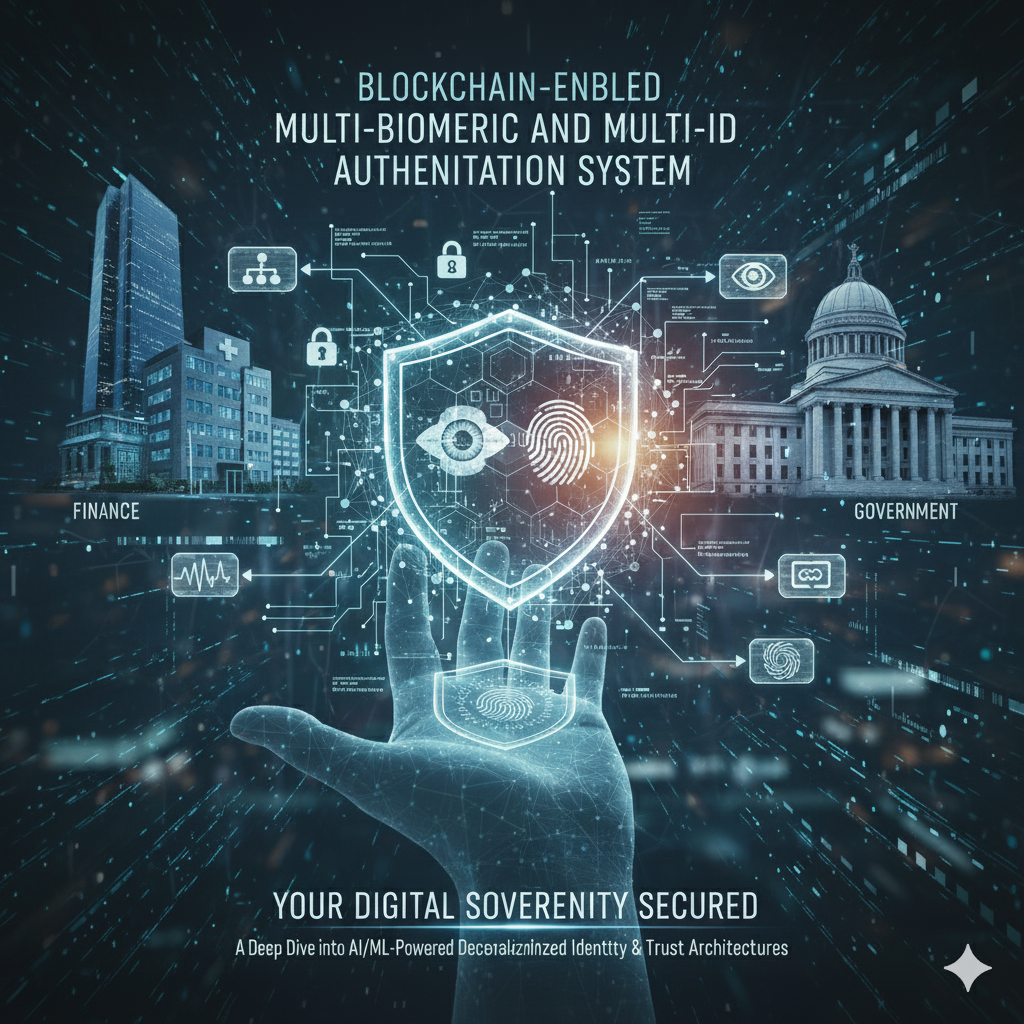
\includegraphics[width=\paperwidth,height=\paperheight]{Gemini_Generated_Image_z6nz4cz6nz4cz6nz.png}%
            }{%
                \fbox{\parbox[c][0.6\paperheight][c]{0.8\paperwidth}{\centering\Large Cover image missing}}
            }%
            \vfill
        }%
    }%
}

%===========================================================
% ===================== CODE HIGHLIGHTING ==================
%===========================================================
\usepackage{listings}
\lstset{
    basicstyle=\ttfamily\small,
    frame=single,
    breaklines=true,
    backgroundcolor=\color{blue!5!white},
    rulecolor=\color{myblue},
    keywordstyle=\color{myblue}\bfseries,
    commentstyle=\color{gray}\itshape,
    stringstyle=\color{orange!80!black}
}

%===========================================================
% ===================== DOCUMENT START ====================
%===========================================================
\begin{document}

%---------------- COVER PAGE ----------------
\begin{titlepage}
  \AddToShipoutPictureBG*{\BackgroundPic}
  \thispagestyle{empty}
  \null
\end{titlepage}
\clearpage

%---------------- TITLE PAGE ----------------
\pagenumbering{roman}
\setcounter{page}{1}
\begin{titlepage}
    \centering
    {\huge\bfseries\headingfont\color{myblue}
        Blockchain-Enabled Multi-Biometric and Multi-ID Authentication System using AI/ML\par}
    \vspace{2.3cm}
    {\large\itshape by \par}
    {\LARGE Jadav Madhavkumar H. \par}
    \vfill
    {\Large A Technical Guide to Secure Identity Management\par}
    \vspace{1cm}
    {\normalsize September 2025 \par}
    \thispagestyle{empty}
\end{titlepage}
\clearpage

%---------------- COPYRIGHT ----------------
\thispagestyle{empty}
\vspace*{\fill}
\begin{center}
  {\large\bfseries Copyright \textcopyright~2025 by Jadav Madhavkumar H.}\par
  \vspace{8pt}
  All rights reserved. No part of this book may be reproduced or transmitted in any form without written permission.
\end{center}
\vspace*{\fill}
\clearpage

%---------------- DEDICATION ----------------
\thispagestyle{empty}
\vspace*{\fill}
\begin{center}
    \textit{To my project guide, for their invaluable support and guidance.}
\end{center}
\vspace*{\fill}
\clearpage

%---------------- TOC & LISTS ----------------
\tableofcontents
\clearpage
\listoffigures
\clearpage

%---------------- ABSTRACT ----------------
\IfFileExists{abstract.tex}{\chapter*{Abstract}
\addcontentsline{toc}{chapter}{Abstract}

% \begin{tcolorbox}[
%   colback=white!98!gray,
%   colframe=techblue!90!black,
%   title=Project Abstract,
%   fonttitle=\bfseries\large,
%   coltitle=black,
%   sharp corners,
%   enhanced,
%   boxrule=1pt,
%   titlerule=0.8pt,
%   drop fuzzy shadow=black!30,
%   left=6mm,
%   right=6mm,
%   top=4mm,
%   bottom=4mm
% ]

\justifying
\setlength{\parskip}{6pt}

The rapid digitalization of services has amplified the need for secure, scalable, and user-friendly authentication mechanisms that transcend the limitations of conventional password or single-factor approaches. 

This project proposes a \textbf{Blockchain-Enabled Multi-Biometric and Multi-ID Authentication System} that leverages the combined power of distributed ledger technology and AI/ML-driven decision models to deliver a robust, tamper-resistant identity verification framework. By integrating multiple biometric modalities—such as \emph{fingerprint, iris, face, and voice recognition}—with government-issued and organizational identity proofs, the system ensures multi-layered trust while reducing the risks associated with spoofing, identity theft, and credential compromise. 

\medskip

\noindent
\textbf{Blockchain} is employed to provide immutable, transparent, and decentralized storage of authentication records, eliminating reliance on a single point of failure. Meanwhile, \textbf{AI/ML algorithms} enhance accuracy through adaptive learning, anomaly detection, and contextual risk scoring. 

The proposed architecture is designed with interoperability, scalability, and privacy-preservation at its core, enabling seamless deployment across domains such as \emph{e-governance, financial services, healthcare, and IoT ecosystems}. This framework not only strengthens cybersecurity resilience but also charts a pathway toward a unified, trustless, and user-centric digital identity infrastructure.

\end{tcolorbox}

}{%
  \begin{center}\textit{Abstract file `abstract.tex' not found.}\end{center}
}
\clearpage

%---------------- MAIN CONTENT ----------------
\pagenumbering{arabic}
\setcounter{page}{1}

% Part I
\part{Understanding the Crisis and Building the Foundations}
\chapter{Introduction}
\chapter{The Crisis of Digital Identity in the Modern Age}

\section{The Great Authentication Paradox: Trusting the Unreliable}
The digital age promised seamless connectivity, yet it is haunted by a paradox: the very tools we use to prove who we are—passwords, PINs, one-time codes—have become the weakest link in the chain. Developed for a time when digital threats were rare and modest, these authentication methods now underpin global finance, healthcare, and communication. They are also at the heart of today's largest security failures.

\subsection*{The Password Problem}
\begin{itemize}
    \item \textbf{Human Fallibility:} Passwords are notoriously hard to remember, leading individuals to take dangerous shortcuts: re-using them across sites, picking simple combinations, or writing them down in unsafe places.
    \item \textbf{The Phishing Epidemic:} Social engineering attacks, especially phishing, are now one of the top ways hackers obtain access—tricking users into willingly revealing passwords.
    \item \textbf{Credential Stuffing:} Once passwords are leaked in a breach, billions are tried against other services, exploiting people’s natural tendency to reuse them.
\end{itemize}

\subsection*{The Fragility of Secondary Methods}
\begin{itemize}
    \item \textbf{PINs and Knowledge-Based Questions:} “Secret” questions are often common knowledge or can be researched online. PINs are short and vulnerable to guessing or shoulder-surfing.
    \item \textbf{One-Time Passwords (OTPs):} Although more advanced, OTPs are still phishable and have their own weaknesses—such as SIM-swapping attacks, where an attacker steals your phone number and intercepts codes.
\end{itemize}

\section{The Catastrophic Consequences: When Identity Becomes a Commodity}
Failed authentication methods have transformed personal data into a currency of crime. Breaches don’t just cost companies money; they turn lives upside down and fuel a shadowy economy where anyone’s identity might be for sale.

\begin{itemize}
    \item \textbf{Escalating Data Breaches:} Over the last decade, massive incidents—like Equifax and Yahoo—have exposed billions of records. The trend isn't slowing.
    \item \textbf{The Dark Web Economy:} Stolen data, including personally identifiable information (PII), payment cards, and even health records, are traded in thriving illicit markets. Cybercriminals amass fortunes exploiting this information.
    \item \textbf{The Human Cost:} The impact goes beyond money—it can ruin credit, destroy reputations, and cause lasting emotional distress for victims, who often spend years untangling the consequences.
\end{itemize}

\section{The Flaw of Centralized Authority: A ``Single Point of Failure''}
Society has long entrusted identity to large institutions—banks, governments, tech giants. Centralized identity management, however, creates attractive, high-value targets for attackers.

\begin{itemize}
    \item \textbf{Centralized Databases as Magnets:} Huge troves of sensitive data are stored in single locations, presenting the perfect honey pot for attackers seeking maximum payoff with a single breach.
    \item \textbf{Lack of Control and Visibility:} Ordinary users rarely know what data is held about them, where, or who accesses it—and have little recourse if something goes wrong.
    \item \textbf{Siloed Identities:} Each service issues a new digital identity. The result is friction (constant sign-ups, password resets) and a fragmented, cumbersome online existence.
\end{itemize}

\section{Biometrics: The Promise and the Pitfall}
Biometrics—fingerprints, faces, voices—were hailed as the future, a way to transcend passwords. The reality is more nuanced.

\begin{itemize}
    \item \textbf{The Problem with Unimodal Biometrics:} Systems relying on a single biometric trait can be defeated: fingerprints lifted from glass, faces spoofed by photos, voices cloned by AI.
    \item \textbf{The Immutability Dilemma:} Unlike a password, you can’t change your fingerprint. If your biometric data is stolen, you can’t ever “reset” your identity.
    \item \textbf{Non-Universality and Environment:} Not all biometrics work for everyone—and even when they do, conditions like dirt, lighting, or background noise can interfere.
\end{itemize}

\section{Towards a New Paradigm: The Rise of Self-Sovereign Identity (SSI)}
To end this cycle of crisis, a new model is gaining traction—one that gives control back to the individual and harnesses the power of cryptography and decentralization.

\begin{itemize}
    \item \textbf{A Shift in Power:} SSI reimagines identity as something we control. Individuals, not institutions, decide what to share, with whom, and when.
    \item \textbf{Decentralized by Design:} Personal data isn’t locked in corporate vaults. Instead, cryptographic proofs and pointers reside on a distributed ledger, outside any single company’s control.
    \item \textbf{Privacy by Default:} Advanced cryptography enables sharing only what is needed—nothing more. No service needs access to your full birth date if all it needs to know is “over 18.”
\end{itemize}

\section{The Next Generation of Authentication: Our Vision}
It is possible to secure digital identity—without sacrificing privacy, usability, or control. This book reveals how the combination of \textbf{blockchain technology}, \textbf{multi-biometrics}, and advanced \textbf{AI/ML} can address the failures outlined above.

\begin{itemize}
    \item \textbf{A Unified, Secure Solution:} By fusing decentralized ledgers with robust biometric systems and intelligent algorithms, we can create a platform that is resilient, privacy-centric, and future-ready.
    \item \textbf{A Glimpse into the Future:} The following chapters chart a path to a world where identity is secure by design—enabling trust in every digital transaction, unlocking new experiences, and restoring confidence in the digital society.
\end{itemize}

% You may add a callout or visual summary here, e.g.:
% \begin{tcolorbox}[colback=techgreen!10!white,colframe=techblue!80!black,title=What Comes Next]
% In the next chapters, we explore the foundational technologies—blockchain, advanced biometrics, and AI—that power this vision.
% \end{tcolorbox}


\chapter{Foundations of Trust: Blockchain and Decentralized Ledgers}

\section{Beyond Buzzwords: What is Blockchain, Really?}
Blockchain technology is often invoked as a panacea, yet few truly understand its transformative underpinnings. At its heart, blockchain is a breakthrough in how trust is established, maintained, and proven in a digital world.

\subsection*{Distributed Ledger Technology (DLT) Explained}
Imagine a shared, ever-growing digital spreadsheet—visible and synchronized for all participants in a network, but not owned or controlled by any single party. This is the core concept of distributed ledger technology (DLT). Unlike conventional databases, where a central authority updates and guards the records, DLT ensures that every participant holds a synchronized copy, and all agree upon changes.

\subsection*{The “Block” and the “Chain”}
Transactions in a blockchain are grouped into “blocks.” Each block references the one before it through a cryptographic hash, creating a chain that is mathematically impossible to alter retroactively without consensus from the network. This chaining mechanism creates an ever-growing, tamper-evident record—what we call the blockchain.

\subsection*{Why Decentralization Matters}
\begin{itemize}
    \item \textbf{Eliminating Middlemen:} Blockchain eliminates the need for a trusted central authority (like a bank or government) to validate records. Parties can transact directly, leveraging the consensus of the network to establish trust.
    \item \textbf{Resilience and Redundancy:} Decentralized networks are inherently robust: even if several nodes go offline or are attacked, the system as a whole continues to function without data loss or corruption.
\end{itemize}

\section{The Pillars of Trust: Core Properties of Blockchain}
The real power of blockchain emerges from a handful of breakthrough characteristics—immutability, transparency, and cryptographic security—that shift the landscape of digital trust.

\subsection*{Immutability: A Record Set in Stone}
Every block added to the chain is sealed with a cryptographic hash tied to the previous block. If anyone attempts to alter any information in a previous block, the hashes for all subsequent blocks change, making tampering instantly obvious to others. For digital identity, this means that enrollment, authentications, and modifications are permanently verifiable, creating a “source of truth” for trust.

\subsection*{The Audit Trail}
Immutability creates a faultless, tamper-proof audit trail—each event is indelibly logged. For identity management, this ensures a clear and irrefutable history for every claim, credential, or status change.

\subsection*{Transparency (Selective) and Verifiability}
On public blockchains, all transactions are visible for inspection. While identity-specific data can be kept private (e.g., via encryption or off-chain storage), the mere existence and validity of a credential can be transparently verified. Later in this book, we’ll see how zero-knowledge proofs let you prove validity without exposing private details—a perfect fit for privacy-preserving digital identity.

\subsection*{Security Through Cryptography}
\begin{itemize}
    \item \textbf{Hashing:} A hash function transforms any data into a unique fixed-length string, which cannot be reversed. This secures data links between blocks and ensures that even the smallest modification stands out.
    \item \textbf{Digital Signatures:} Public-key cryptography lets users demonstrate ownership or approval without revealing private information. Used for signing transactions, it guarantees authenticity and non-repudiation.
\end{itemize}

\section{Orchestrating Agreement: Blockchain Consensus Mechanisms}
For a decentralized system to work, network participants (nodes) must agree on changes—this universal truth is achieved through consensus algorithms.

\subsection*{Proof of Work (PoW)}
Participants (“miners”) solve complex cryptographic puzzles to win the right to add blocks. This process is energy-intensive, limiting throughput, but offers security that’s difficult to subvert (as seen in Bitcoin and early Ethereum).

\subsection*{Proof of Stake (PoS)}
Validators are selected to add blocks based on the amount of cryptocurrency they are willing to “stake” as collateral. It conserves energy and enables higher transaction speeds. Security is maintained by threatening “slashing” (loss of staked currency) as a penalty for malicious actions.

\subsection*{Permissioned Consensus (e.g., PBFT, Raft)}
For enterprise and consortium blockchains, consensus is achieved among a select group of known, authorized participants. Examples include Practical Byzantine Fault Tolerance (PBFT) and Raft. These approaches offer higher speed, lower cost, and tailored privacy—perfect for regulated industries and private networks.

\section{The Code of Trust: Smart Contracts}
Smart contracts extend the blockchain’s capability with programmable, self-executing agreements.

\begin{itemize}
    \item \textbf{Definition:} A smart contract is a program that runs when predetermined conditions are met. The rules are transparent and immutable—the contract executes itself when requirements are satisfied, without any intermediary.
    \item \textbf{Automation:} Functions range from simple transfers (“pay if delivered”) to complex workflows that might issue or revoke digital credentials automatically.
    \item \textbf{Role in Digital Identity:} Smart contracts can automate credential issuance, manage access rules (“who can see what”), and even handle revocation or updates to attributes—all enforced by code, not by trust in a human administrator.
\end{itemize}

\section{Why Blockchain is Indispensable for Secure and Auditable Identity}
Bringing these elements together, blockchain is not just a promising option—it is foundational for truly secure, auditable, and privacy-respecting digital identity:

\begin{itemize}
    \item \textbf{Decentralization:} Sidesteps the “single point of failure” of centralized systems, directly mitigating the attack vectors detailed in Chapter 1.
    \item \textbf{Immutability:} Permanently and publicly records every credential, transaction, or change, making fraud nearly impossible and auditing effortless.
    \item \textbf{Transparency vs. Privacy:} Selective transparency (with tools like zero-knowledge proofs) ensures the system is accountable, but never compromises sensitive personal data.
    \item \textbf{Smart Contracts:} Powers trusted automation of credential management, validation, and access control, reducing reliance on manual processes and the potential for error or abuse.
\end{itemize}

\section{Public vs. Permissioned Blockchains: Choosing the Right Foundation}
Not every blockchain is fit for sensitive identity information. The choice of platform dictates privacy, scalability, and governance.

\subsection*{Public Blockchains (e.g., Ethereum, Bitcoin)}
\begin{itemize}
    \item \textbf{Characteristics:} Open to anyone, highly decentralized, pseudonymous, with all transactions visible to the public.
    \item \textbf{Pros:} Censorship-resistant, robust global infrastructure.
    \item \textbf{Cons:} High fees, lower throughput, and the fact that all data (even encrypted) is visible—restricting use for direct storage of personal data such as PII.
\end{itemize}

\subsection*{Permissioned Blockchains (e.g., Hyperledger Fabric, R3 Corda)}
\begin{itemize}
    \item \textbf{Characteristics:} Network membership is restricted to known, vetted entities; consensus is reached through faster, more private means among trusted nodes.
    \item \textbf{Pros:} High scalability, fine-grained privacy, compliance-friendly governance, and enterprise integration.
    \item \textbf{Cons:} Somewhat less decentralized; requires a trust model among participating organizations.
\end{itemize}

\subsection*{The Rationale for Permissioned Blockchains in DMID}
Given the requirements for privacy, scalability, and enterprise alignment in digital identity management, permissioned blockchains such as Hyperledger Fabric are the natural choice. They offer:
\begin{itemize}
    \item Data privacy through private channels and selective disclosure.
    \item High throughput and customizable governance.
    \item Seamless integration with existing organizational infrastructure and compliance controls.
\end{itemize}

% Optionally, include figures or diagrams to illustrate public vs. permissioned blockchain differences or consensus mechanisms.

% \begin{figure}[h]
%   \centering
%   \includegraphics[width=0.7\textwidth]{blockchain_layers.png}
%   \caption{Public vs. Permissioned Blockchain Architecture}
% \end{figure}


\chapter{The Power of You: Multi-Biometrics and Intelligent Authentication}

\section{The Human Signature: A Foundation in Biometric Identity}

\subsection{Defining Biometrics: From Measurement to Authentication}
Biometric authentication represents a true paradigm shift in digital identity. It moves the field away from what we \emph{know} (passwords) and what we \emph{have} (tokens), toward what we \emph{are}. Biometrics is the science of measuring the unique physical and behavioral characteristics of individuals for the purposes of identification and verification.

Biometric systems operate in two primary modes:
\begin{itemize}
    \item \textbf{Identification (1:N):} The system compares a fresh biometric against all enrolled templates in its database to find a match.
    \item \textbf{Verification (1:1):} The system checks whether the fresh biometric matches a single, pre-enrolled template, confirming or denying a claimed identity.
\end{itemize}

The robustness of these systems arises from the uniqueness and permanence of human traits—qualities that make biometric authentication vastly harder to compromise than traditional security factors.

\subsection{The Spectrum of Biometric Modalities: Physiological vs. Behavioral}
Biometric traits are grouped into physiological and behavioral modalities, each with its own operational strengths.

\begin{itemize}
    \item \textbf{Physiological biometrics:} Rely on anatomical features (fingerprints, face, iris, veins, etc.). Generally permanent and useful for high-assurance identity verification, often paired with trusted documents.
    \item \textbf{Behavioral biometrics:} Involve the distinctive ways a person interacts with the world (voice, gait, keystroke dynamics, etc.), excelling at frictionless, continuous authentication behind the scenes.
\end{itemize}

A layered security model emerges: use physiological traits for strong initial setup, then continuously monitor a session with passive behavioral traits, combining convenience and security.

\subsubsection{Physiological Traits: The Immutable Self}
\begin{itemize}
    \item \textbf{Fingerprint Recognition:} Unique friction ridge patterns; modern capacitive sensors resist spoofing.
    \item \textbf{Facial Recognition:} Analyzes facial geometry using AI to counteract pose and lighting variations.
    \item \textbf{Iris \& Retina Scanning:} Ultra-unique, stable eye patterns; iris is easy and non-intrusive, retina scanning is highly secure but less user-friendly.
    \item \textbf{Vein Recognition:} Scans subdermal vein patterns, extremely difficult to forge.
\end{itemize}

\subsubsection{Behavioral Traits: The Dynamic Self}
\begin{itemize}
    \item \textbf{Voice Recognition:} Leverages rhythm, pitch, and cadence.
    \item \textbf{Gait Analysis:} Measures how a person walks—speed, stride, body posture.
    \item \textbf{Keystroke Dynamics:} Captures timing and pressure of typing, offering continuous monitoring.
\end{itemize}

\begin{table}[h]
\centering
\caption{Comparison of Biometric Modalities}
\begin{tabular}{|l|c|c|c|c|c|c|c|}
\hline
\textbf{Modality} & \textbf{Type} & \textbf{Universality} & \textbf{Permanence} & \textbf{Uniqueness} & \textbf{Accuracy} & \textbf{Acceptability} & \textbf{Cost} \\
\hline
Fingerprint & Physio & Mod & High & High & High & High & Low \\
Face & Physio & High & Mod & High & High & Very High & Low \\
Iris & Physio & High & Very High & Very High & Very High & Mod & High \\
Vein & Physio & High & Very High & Very High & Very High & Mod & Mod \\
Voice & Behav & High & Low & Mod & Mod & High & Low \\
Gait & Behav & High & Low & Low & Low & Very High & Low \\
Keystrokes & Behav & High & Low & Low & Low & Very High & Very Low \\
\hline
\end{tabular}
\end{table}

\section{The Fallibility of a Single Factor: Unimodal Biometric Limitations}

\subsection{Inherent Vulnerabilities: Non-Universality and Noisy Data}
Unimodal systems suffer from:
\begin{itemize}
    \item \textbf{Non-Universality:} Not all modalities work for all people (e.g., worn fingerprints, cultural constraints).
    \item \textbf{Noisy Data:} Sensor/environmental issues (poor lighting, dirt, humidity) can cause misreadings and increase false rejections.
\end{itemize}

\subsection{The Threat of Spoofing and Presentation Attacks}
\textbf{Presentation attacks} include using artificial fingerprints (made of gelatin or silicone), photos for facial spoofing, or printed irises and custom lenses.

\subsubsection{The Rise of Deepfakes and AI-Powered Spoofing}
AI-powered deepfakes generate hyper-realistic fake biometric samples. GANs and other neural networks can create forgeries that mimic nuance and bypass traditional liveness checks—a challenge that grows with each iteration of generative AI.

\section{The Synergy of Self: The Strategic Advantage of Multi-Biometrics}

\subsection{A Multi-Layered Defense: Enhanced Security and Robustness}
Multimodal systems compound security by requiring the attacker to spoof multiple traits at once—each captured and processed by distinct sensors and algorithms. This layering multiplies difficulty and greatly reduces the chance of a successful breach.

\subsection{Overcoming Unimodal Challenges: Accuracy, Reliability, and User Experience}
By fusing multiple modalities, these systems mitigate environmental, sensor, or user-specific limitations of any single biometric. Redundancy reduces false rejections, improves universality, and creates a smoother, more reliable user experience.

\subsection{The Economic and Operational Case for Multimodal Systems}
Though initially more costly, multimodal systems decrease long-term risk and operational loss thanks to far greater fraud resistance—they are essential in high-value, high-security environments.

\section{The Intelligent Architectures of Fusion: A Technical Deep Dive}

There are four levels of biometric fusion:
\begin{table}[h]
\centering
\caption{Comparison of Biometric Fusion Levels}
\begin{tabular}{|l|l|l|l|l|l|l|}
\hline
\textbf{Fusion Level} & \textbf{Stage} & \textbf{Information} & \textbf{Complexity} & \textbf{Accuracy} & \textbf{Advantage} & \textbf{Drawback} \\
\hline
Sensor      & Raw Data  & High  & Very High & Highest    & Max info   & Hard to implement \\
Feature     & Post-Feature & High & High & High & Rich info      & Incompatible data \\
Score       & Post-Match  & Med  & Med & Med & Good balance   & Score normalization \\
Decision    & Final      & Low   & Low & Lowest     & Simple        & Least accurate \\
\hline
\end{tabular}
\end{table}

\subsection{Sensor-Level Fusion}
Combines raw data before processing. Offers rich info but hard to implement.

\subsection{Feature-Level Fusion}
Merges extracted feature vectors into one. Needs careful normalization; high dimensionality can add processing overhead.

\subsection{Score-Level Fusion}
Combines independent modal scores (e.g., sum/product/weighted voting) for the final decision. The most widely used approach due to its balance of information, simplicity, and accuracy.

\subsection{Decision-Level Fusion}
Each modality issues a binary accept/reject, and a fusion rule (e.g., majority vote) delivers the final verdict. Simple but least informative.

\section{The Neural Revolution: AI/ML as the Engine of Intelligent Authentication}

\subsection{The Foundation: Machine Learning in Biometrics}
AI and ML have automated the extraction and fusion of biometric features, greatly improving real-time recognition, adaptability, and fraud detection.

\subsection{Deep Learning for Feature Extraction and Pattern Recognition}
\begin{itemize}
    \item \textbf{Convolutional Neural Networks (CNNs):} State-of-the-art for physiologic traits (faces, fingerprints, irises); extract multi-scale features robust to noise, lighting, and pose variation.
    \item \textbf{Recurrent Neural Networks (RNNs)/LSTM:} Best for behavioral time-series (gait, voice, keystroke dynamics), learning complex, long-term dependencies.
\end{itemize}
The same advances that fuel deepfake creation are leveraged for anti-fraud by learning the subtle cues of real vs. generated samples. These models continuously improve, responding to new attack vectors.

\section{The Unblinking Eye: The Crucial Role of Liveness Detection}

\subsection{What is Liveness Detection and Why it is a Game-Changer}
Liveness detection (Presentation Attack Detection, PAD) ensures biometric input is from a live user, not a replica—critical against spoofing and deepfakes.

\subsection{Active Liveness Detection: User-Centric Security}
Requires explicit user action (e.g., blink, smile, turn head). Enhances security but can disrupt UX.

\subsection{Passive Liveness Detection: The Seamless Experience}
Analyzes images/videos passively for authenticity by detecting micro-movements, natural textures, and light. Frictionless, scalable, and user-friendly.

\subsection{Hybrid Models}
Blend active and passive checks—e.g., a selfie with a quick gesture. Designed to maximize security and usability based on use case.

\begin{table}[h]
\centering
\caption{Comparison of Liveness Detection Techniques}
\begin{tabular}{|l|c|c|c|c|}
\hline
\textbf{Technique} & \textbf{User Interaction} & \textbf{User Experience} & \textbf{Security} & \textbf{Use Cases} \\
\hline
Active & Yes & Disruptive, Less convenient & High & High-security, Onboarding \\
Passive & No & Seamless, Frictionless & Mod-High & Banking, E-commerce \\
Hybrid & Yes (quick task) & Balanced & High & Sensitive transactions \\
\hline
\end{tabular}
\end{table}

\section{Real-World Implementation and The Path Forward}

\subsection{Case Studies in Banking and Healthcare}
\begin{itemize}
    \item \textbf{Finance:} Biometrics and behavioral traits provide secure logins, fraud prevention, and continuous risk monitoring.
    \item \textbf{Healthcare:} Ensures accurate, privacy-protecting access to medical records; biometrics at bedside prevent errors and fraud.
\end{itemize}

\subsection{Ethical Considerations: Privacy, Data Security, and Regulation}
Despite their security strengths, biometrics introduce critical risks: once stolen, a biometric cannot be changed. Risks of mass surveillance, “function creep,” or data misuse have led to strong privacy laws (like BIPA). Successful implementation demands robust consent, transparency, and clear policies for data retention and usage.

\section*{Conclusion}
The move from passwords to unimodal biometrics, and now to AI-powered multimodal frameworks, is driven by the dual challenges of security and usability in a digital world. Intelligent fusion and sophisticated liveness detection powered by AI/ML form the core of the future of authentication, making the system resilient, adaptive, and centered on both security and privacy. This future will not rely on a single magic trait, but on a dynamic, learning ecosystem—balanced with robust ethics and law.


\chapter{Designing the Decentralized Multi-Biometric Identity System (DMIDS)}

\section{Introduction: The Foundational Paradigm Shift}
Digital identity is at a crossroads, evolving from centralized models where a single authority managed your credentials, through federated and user-centric approaches, toward truly self-sovereign identity (SSI). SSI—where each individual owns and fully manages their digital identity—redistributes power away from centralized custodians, drastically reducing risk and enabling compliance with modern data protection regulations (\emph{e.g.}, GDPR, eIDAS).

A decentralized multi-biometric identity system (DMID) is the architectural answer to traditional vulnerabilities: it uses cryptography, user-side security, and modular architecture to empower end users and minimize central data silos. Two enabling primitives form its core:
\begin{itemize}
    \item \textbf{Decentralized Identifiers (DIDs):} Globally unique, cryptographically verifiable identifiers controlled by the user, not any authority.
    \item \textbf{Verifiable Credentials (VCs):} Cryptographically secured, tamper-proof digital attestations (e.g., ``over 18'', ``university graduate'') controlled and selectively disclosed by the user.
\end{itemize}
Together, DIDs and VCs lay the foundation for portable, private, and user-controlled identity.

\section{High-Level System Architecture and Component Blueprint}
DMID is built from modular, decoupled components for lifecycle security and user control.

\subsection{Conceptual Architecture Diagram}
\begin{figure}[h]
    \centering
    % Replace filename with your actual diagram
    \includegraphics[width=0.82\textwidth]{dmid_architecture.png}
    \caption{DMID High-Level Architecture: Data Flow, Trust Layers, and On-/Off-Chain Separation}
\end{figure}

\begin{itemize}
    \item \textbf{User Device \& Digital Wallet:} Biometric capture (camera, fingerprint, etc.); biometric processing engine for template extraction; secure wallet for storage of DIDs, VCs, and private keys.
    \item \textbf{Identity Provider (IdP):} Trusted for initial proofing and credential issuance (may use AI/OCR, internal biometrics, etc.).
    \item \textbf{Service Provider (SP):} Verifies user identity, cryptographically validates credentials with no need to contact the issuer.
    \item \textbf{Blockchain Network:} Anchors proofs (DIDs, VC hashes, revocation registries), without storing PII—serves as public notary for cryptographic proofs and state.
\end{itemize}

\subsection{Component Roles and Technical Interactions}
\begin{itemize}
    \item Biometric capture and template creation is always off-chain (either on user device or a secure IdP system).
    \item Raw biometrics $\rightarrow$ biometric template $\rightarrow$ template hashed (cryptographic hash).
    \item Blockchain records root hashes (e.g., Merkle Tree), credential references, and DIDs—never raw PII.
    \item A compromised actor would need to breach multiple discrete systems, making DMID vastly more secure by design.
\end{itemize}

\section{The Lifecycle of a Digital Identity}

\subsection{Enrollment and Credential Issuance}
\begin{itemize}
    \item User provides a government ID scan and biometrics on their device.
    \item IdP OCR/AI parses ID, creates biometric template, hashes it, and builds a Merkle Tree of attributes.
    \item Merkle root hash stored on-chain; IdP issues cryptographically signed VC to user wallet.
\end{itemize}

\subsection{Verification and Authentication}
\begin{itemize}
    \item User presents relevant VC and live biometric.
    \item SP (Verifier) checks:
    \begin{enumerate}
        \item Issuer's DID/public key from chain.
        \item VC digital signature.
        \item Revocation status (on-chain registry).
        \item Live biometric against off-chain stored template; optionally, selective disclosure via zero-knowledge proofs.
    \end{enumerate}
\end{itemize}

\subsection{Ongoing Management and Revocation}
\begin{itemize}
    \item Users can revoke credentials directly from their wallet.
    \item Issuer updates revocation status on-chain.
    \item Enables dynamic control: users manage consent and access without intermediaries.
\end{itemize}

\begin{table}[h]
\centering
\caption{Digital Identity Lifecycle: Actors, Inputs, Artifacts, Objectives}
\begin{tabular}{|l|l|l|l|l|}
\hline
\textbf{Phase} & \textbf{Actors} & \textbf{Input} & \textbf{Output} & \textbf{Objective} \\
\hline
Enrollment & Holder, IdP & PII, ID, Biometric & VC, Template (off-chain), Merkle hash (on-chain), DID & Establish trust, minimize PII held by IdP \\
Verification & Holder, Verifier & VC, live biometric & Proof of claim, match score & Private, instant, secure auth \\
Ongoing Mgmt & Holder, Issuer & Revoke/update request & On-chain status, updated VC & User control of identity \\
\hline
\end{tabular}
\end{table}

\section{Data Strategy: The On-Chain vs. Off-Chain Paradigm}

\subsection{The Case for Off-Chain Biometric Data Storage}
\begin{itemize}
    \item On-chain storage of biometrics is forbidden—immaturity, privacy law conflicts, and permanence risks (cannot be deleted/erased).
    \item Most personal and biometric data is stored off-chain (user device, secure cloud, or trusted enclave).
    \item Templates, documents, and sensitive datasets are only referenced on-chain via cryptographic hashes.
\end{itemize}

\subsection{The On-Chain Role: Immutable Proofs and Integrity Anchoring}
\begin{itemize}
    \item On-chain, store only small, critical, immutable proofs:
    \begin{itemize}
        \item DIDs (no PII)
        \item Hashes of biometric templates / credentials
        \item Merkle Tree roots for bundling attributes
    \end{itemize}
    \item This maximizes auditability and integrity, with zero risk of PII exposure or breach.
\end{itemize}

\begin{table}[h]
\centering
\caption{On-Chain vs. Off-Chain Storage Comparison}
\begin{tabular}{|l|l|l|}
\hline
\textbf{Criterion} & \textbf{On-Chain} & \textbf{Off-Chain} \\
\hline
Cost & Prohibitively high & Low for large files \\
Scalability & Very limited & Very high \\
Data Integrity & Perfect & Needs hash verification \\
Privacy/Security & Visible, immutable & Controllable, erasable \\
Use Cases & Proofs, DIDs, hashes & Biometrics, documents \\
\hline
\end{tabular}
\end{table}

\section{Addressing Scalability and Performance Challenges}
The \textbf{Blockchain Trilemma} (decentralization, security, scalability) affects all identity designs. DMID leverages a hybrid architecture:
\begin{itemize}
    \item \textbf{Layer 2 (L2) Solutions:} Rollups (Optimistic, ZK) batch hundreds of verifications off-chain and anchor results on-chain—increasing throughput and lowering cost.
    \item \textbf{Sidechains:} Offload high-volume processing, bulk storage, and verification processes.
    \item \textbf{Merkle Trees:} Aggregate many proofs/attributes for a single on-chain anchor.
    \item \textbf{Sharding:} Parallelizes blockchain operations for very high throughput.
\end{itemize}

\section{Trust Models in a Decentralized Environment}

\subsection{The Trust Triangle: Issuer, Holder, Verifier}
\begin{itemize}
    \item \textbf{Issuer:} Issues (signs) credentials—e.g., governments, universities, trusted KYC providers.
    \item \textbf{Holder:} Individual who owns and controls VCs/DIDs in their wallet.
    \item \textbf{Verifier:} Entity that needs to verify a claim; relies solely on cryptographic proofs, not the issuer’s word.
\end{itemize}
This cryptographic ``triangle of trust'' is validated by protocols, signatures, and immutable blockchain records, not by phone calls or emails to a trusted authority.

\subsection{DIDs and VCs: The Building Blocks of Trust}
\begin{itemize}
    \item DIDs: Self-sovereign unique identifiers, public keys, anchored on the chain.
    \item VCs: Signed digital claims about DIDs, packaged for selective disclosure.
    \item Trust is based on signature chains—Verifiers validate credentials without direct Issuer contact.
\end{itemize}

\subsection{The Role of Zero-Knowledge Proofs (ZKPs)}
Zero-knowledge proofs (especially zk-SNARKs) allow users to prove possession of an attribute or claim (e.g., ``over 18'') without revealing any of the sensitive data itself.  
This enables true data minimization, granular consent, and private authentication—signature validation and proof checks are all a verifier needs.

\section*{Conclusion}
DMID embodies the new paradigm of distributed, user-centric identity: modular, privacy-centric, and performance-optimized. By decoupling on-chain proofs from off-chain sensitive data, supporting scalable verification with Layer 2 and cryptographic primitives, and redefining the trust model using DIDs, VCs, and ZKPs, DMID emerges as a strategic, compliant, and technically superior approach to digital identity in the 21st century.


\chapter{Cryptographic Engineering for Ultimate Privacy and Security}

\section{The Foundation of Trustless Verification: Merkle Trees}

A Merkle tree (hash tree) is a hierarchical data structure used to efficiently and securely verify the integrity of large datasets. Each leaf node contains the hash of a data block, while non-leaf nodes contain the hash of their children's hashes. This recursion yields a single "Merkle root," representing the integrity of the entire tree.

This design allows rapid, efficient, logarithmic-time verification of any data block. Light clients can verify transactions with Merkle proofs rather than downloading entire datasets—a foundation of public blockchain scalability and trust minimization.

\subsection{Merkle Proofs: Enabling Lightweight and Private Verification}
A Merkle proof (or Merkle path) provides evidence that a particular datum belongs to a set without revealing the entire dataset. The proof comprises the relevant data block, its hash, and the hashes of its siblings up to the root. A Verifier recomputes the sequence to validate the commitment. This is crucial for selective disclosure of personal attributes—e.g., proving age eligibility without exposing the actual birthdate.

\subsection{Real-World Applications and Engineering Context}
Merkle trees are standard in blockchains (to aggregate thousands of transactions in a block), anti-entropy protocols in distributed databases, and peer-to-peer file systems for integrity checks.

\subsection{Engineering Challenges and Advanced Architectures}
Traditional Merkle trees are costly to update or extend for dynamic data, leading to structures like Merkle Patricia Tries (used in Ethereum) that blend trie and hash logic for efficient dynamic operations.

\section{Proving Without Revealing: The Paradigm of Zero-Knowledge Proofs (ZKPs)}

A Zero-Knowledge Proof (ZKP) allows a Prover to convince a Verifier of a statement's truth without revealing anything but that truth. ZKPs feature:
\begin{itemize}
    \item \textbf{Completeness}: If the statement is true, an honest Prover can convince an honest Verifier.
    \item \textbf{Soundness}: If a statement is false, a dishonest Prover cannot convince the Verifier except with negligible probability.
    \item \textbf{Zero-Knowledge}: The Verifier learns nothing beyond the validity of the statement.
\end{itemize}

\subsection{A Spectrum of ZKPs: Interactive vs. Non-Interactive}
Interactive ZKPs (iZKPs) require multiple communication rounds between Prover and Verifier. Non-interactive ZKPs (NIZKPs) need just a single message—enabling asynchronous, large-scale verifications ideal for blockchains.

\subsection{Leading-Edge Implementations: ZK-SNARKs and ZK-STARKs}
\begin{table}[h]
\centering
\caption{Comparison of ZKP Types}
\begin{tabular}{|l|c|c|}
\hline
\textbf{Criterion} & \textbf{ZK-SNARKs} & \textbf{ZK-STARKs} \\
\hline
Proof Size & Short & Larger \\
Verification Speed & Very Fast & Fast \\
Trusted Setup & Required & Not Needed (Transparent) \\
Quantum Resistant & No & Yes \\
Scalability & Good (specific) & Excellent (general) \\
Underlying Crypto & Elliptic Curves & Hashes/\newline FFTs \\
\hline
\end{tabular}
\end{table}

\subsection{Applications for Private Identity and Data}
ZKPs power selective disclosure in identity—proving a claim (over 21, has license, is citizen) without exposing personal data. They underpin private voting, confidential transactions, and scaling (as in ZK-Rollups).

\section{Securing Computation: The Promise of Homomorphic Encryption (HE)}

Homomorphic Encryption enables operations on ciphertexts; decrypting the result yields what would have arisen from operating on the plaintext. Types:
\begin{itemize}
    \item \textbf{PHE (Partially)}: One operation permitted (e.g., only addition or only multiplication)
    \item \textbf{SHE (Somewhat)}: Limited computation depth
    \item \textbf{FHE (Fully)}: All operations permitted, any computation
\end{itemize}

\subsection{Practical Application: Secure Biometric Matching}
Encrypted biometric templates can be matched directly, allowing for privacy-preserving authentication where the comparison is never performed on unencrypted data.

\subsection{Engineering Challenges and the Path to Adoption}
Despite privacy power, HE is resource-intensive and slow, with large ciphertext expansion. Good key management is essential, and present-day HE is practical mainly in limited, targeted roles.

\subsection{Synergy with Other Privacy-Enhancing Technologies (PETs)}
\begin{table}[h]
\centering
\caption{Comparison: PETs for Secure Computation}
\begin{tabular}{|l|l|l|l|}
\hline
\textbf{Technology} & \textbf{Use Case} & \textbf{Key Advantage} & \textbf{Limitation} \\
\hline
HE & Encrypted computation & Utility with privacy & High overhead \\
Secure MPC & Joint computations & Often faster than FHE & Requires coordination \\
Differential Privacy & Data analysis/statistics & Mathematically proven & Result utility trade-off \\
Federated Learning & ML model training & Keeps data local & Still susceptible to inference \\
\hline
\end{tabular}
\end{table}

\section{The Pillars of Integrity and Authentication: Hashing and Digital Signatures}

\subsection{Cryptographic Hashing for Data Integrity}
Hashes map arbitrary data to a fixed-size output, with these properties:
\begin{itemize}
    \item Determinism: Same input $\rightarrow$ same output
    \item Pre-image resistance: Cannot infer input from output
    \item Collision resistance: No two inputs cause the same output
\end{itemize}
Used for file integrity, Merkle tree construction, and as the core of digital signatures.

\subsection{Digital Signatures: A Non-Repudiable Assurance}
Digital signatures use private/public key pairs for authentication and non-repudiation. The sender hashes a message and encrypts the hash with their private key, the receiver verifies by decrypting with the sender's public key and matching the hash.

\subsection{A Synergistic Relationship}
Hashing provides compact data commitment, and digital signatures bind identity and intent to that data for integrity, authentication, and non-repudiation.

\begin{table}[h]
\centering
\caption{Hashing vs. Digital Signatures}
\begin{tabular}{|l|c|c|}
\hline
\textbf{Characteristic} & \textbf{Hashing} & \textbf{Digital Signatures} \\
\hline
Type & One-way & Two-way \\
Purpose & Integrity & Auth., Integrity, Non-repudiation \\
Key Principle & Irreversibility & Public/private key \\
Requirement & Hash function & Private key, hash \\
\hline
\end{tabular}
\end{table}

\section{The Decentralized Revolution: Key Management for User Sovereignty}

\subsection{The Problem with Centralized Key Management}
Centralized key management puts all trust—and risk—on single authorities, making them high-value attack targets.

\subsection{Principles of Decentralized Key Management}
Decentralized Key Management Systems (DKMS) spread key authority across a peer network, greatly increasing resilience and security.

\subsection{Public-Key Crypto in Decentralized Identity (DIDs)}
DID systems rely on public/private key pairs, with DIDs (identifiers) derived from public keys and recorded on-chain. The Issuer, Holder, and Verifier each play essential roles:
\begin{itemize}
    \item \textbf{Issuer:} Issues and signs credentials
    \item \textbf{Holder:} Controls credentials, stores private key securely
    \item \textbf{Verifier:} Checks credentials via public key on-chain, never needing direct confirmation from the Issuer
\end{itemize}

\subsection{Ensuring Security of the Private Key}
While DKMS removes system-level failures, key management moves the risk to the end-user: the security of one's digital life depends on safe local key storage. Advanced wallets, HSMs, or multi-party techniques are needed; identity-based cryptography (IBC) sacrifices sovereignty by re-introducing a trusted third party.

\section*{Conclusion and Future Outlook}
Leading-edge cryptographic primitives, applied thoughtfully and in synergy, transform the way we structure, protect, and selectively share sensitive data in decentralized ecosystems. As power shifts to end-users, future work will focus on advancing PET performance, hardware acceleration, and hybrid models with AI/ML—ensuring that privacy and user sovereignty remain the default, not the exception.


%===========================================================
% Chapter 6: The AI/ML Engine: Fusion, Liveness, and Adaptive Security
%===========================================================

\chapter{The AI/ML Engine: Fusion, Liveness, and Adaptive Security}

\section{The Art of Combination: AI for Biometric Fusion}

The integration of artificial intelligence (AI) and machine learning (ML) has advanced multimodal biometric systems beyond simply collecting multiple data points. At the core of this advancement is the use of intelligent algorithms to fuse data from different biometric sources, enabling a more robust, accurate, and secure authentication decision than any single modality could provide alone. This process, known as fusion, can occur at various stages, but score-level fusion is a particularly common and effective method. It involves each biometric modality---such as a fingerprint or a facial scan---being processed independently to produce its own matching score. These individual scores are then combined into a single, composite score to make the final authentication decision. A variety of machine learning algorithms are employed for this task, each with a distinct approach to consolidating the data.

\subsection{Biometric Fusion Algorithms}

\textbf{Gaussian Mixture Models (GMMs):} GMMs are a form of Bayesian classification used for probabilistic decision-making. They model the distribution of scores for genuine users and impostors as a mixture of Gaussian (bell-curve) distributions. When a new set of scores is presented, the system calculates the probability that these scores belong to the ``genuine'' distribution versus the ``impostor'' distribution. This approach allows the system to make a highly probable decision based on a nuanced understanding of the score data.

\textbf{Artificial Neural Networks (ANNs):} ANNs, including more complex deep learning models, can be trained to recognize intricate patterns in the biometric scores. In a fusion context, an ANN can be trained on a large dataset of genuine and impostor scores from multiple modalities. The network learns to weigh each score's contribution and identify non-linear relationships between them. For instance, in one study, an ANN was used to group input pixels from a combination of face and fingerprint recognition into different clusters, providing an accurate fused result.

\textbf{Support Vector Machines (SVMs):} SVMs are powerful supervised learning algorithms that are trained on data to find an optimal decision boundary that separates genuine users from impostors. In a biometric fusion application, the SVM takes the scores from each modality as inputs and classifies the user based on where those scores fall in relation to this boundary. The algorithm is particularly effective in cases where the data is not easily separable, as it can find a complex, non-linear boundary to maximize the accuracy of the final decision.

%-----------------------------------------------------------
\section{The DeepFake Countermeasure: Liveness Detection with Deep Learning}

As biometric systems have become more prevalent, so too have the threats designed to circumvent them. Modern systems are not just susceptible to simple photo or video attacks; they face advanced threats like AI-generated deepfakes and sophisticated 3D masks. Liveness detection, also known as Presentation Attack Detection (PAD), is a critical line of defense that verifies whether the biometric sample is from a real, live person or a fake replica.

\subsection{Deep Learning for Anti-Spoofing}

AI/ML-based liveness detection systems are trained on vast datasets of both real and fake biometric samples to learn the subtle patterns that distinguish genuine from fraudulent inputs. Deep learning models, particularly Convolutional Neural Networks (CNNs), are highly effective for this purpose because of their ability to analyze visual data for signs of life. These models can identify a wide range of spoofing artifacts, such as:

\begin{itemize}
    \item \textbf{Skin Texture and Reflection:} CNNs can detect minute details like natural skin texture, depth information, and light reflection patterns that are nearly impossible for a fake image or mask to replicate.
    \item \textbf{Micro-movements:} Liveness detection systems analyze subtle, involuntary movements like blinks, micro-expressions, or head turns, which are tell-tale signs of a live person. These natural motions are difficult to mimic with a static photo or even a video replay.
    \item \textbf{Deepfake Anomalies:} Advanced systems can be trained to spot the ``moir\'e noise'' and ``unexpected shadows'' often present in deepfake media. They can also detect subtle differences in synthesized media, such as inconsistent facial expressions or unusual audio patterns.
\end{itemize}

\subsection{Active vs. Passive Liveness Detection}

Liveness detection can be implemented in two primary ways, each with a different user experience:

\begin{itemize}
    \item \textbf{Active Liveness Detection:} This method requires the user to perform a specific action, such as smiling, blinking, or turning their head, in response to a prompt from the system. While this challenge-response approach is generally more difficult for a fraudster to spoof, it can be less convenient for the user and may lead to a more cumbersome authentication process.
    \item \textbf{Passive Liveness Detection:} This non-intrusive approach works in the background without requiring any user action. The system silently analyzes a selfie or video frame for subtle signs of life using advanced computer vision and machine learning. It is often considered more user-friendly and scalable, especially for remote identity verification.
\end{itemize}

A hybrid approach that combines elements of both active and passive detection can be a powerful countermeasure against a wide range of attacks.

%-----------------------------------------------------------
\section{Proactive Defense: Anomaly Detection and Adaptive Security}

The most advanced AI-powered biometric systems are not just reactive---they are proactive. By continuously monitoring user behavior, they can detect subtle anomalies that may indicate a security threat or a presentation attack in real time.

\subsection{Anomaly Detection}

AI systems create a dynamic profile of a user's normal behavior by analyzing a continuous stream of biometric and contextual data. This can include behavioral biometrics like typing speed, rhythm, and pressure, as well as mouse movements and navigation patterns. Once a baseline is established, the system constantly monitors for any significant deviations from this established pattern. For example, a sudden change in typing speed or a login from a new, unfamiliar device or location can trigger a fraud alert. This approach provides a continuous, frictionless authentication layer that operates in the background throughout a user's session, a powerful feature for detecting account takeovers and insider threats.

\subsection{Adaptive Security}

Adaptive security leverages these anomaly detection capabilities to create a flexible, self-improving defense mechanism. The system learns and adapts over time, using new data to improve its accuracy and performance. When a potential threat is detected, the system can automatically adjust its security protocols in real time. This might involve:

\begin{itemize}
    \item \textbf{Step-up Authentication:} If an anomaly is detected, the system can dynamically request an additional form of verification, such as a one-time passcode or a secondary biometric check.
    \item \textbf{Context-Based Triggers:} A system in the banking sector might trigger a more stringent verification process if a user attempts to make a large transaction from a new device, even if the initial biometric login was successful.
\end{itemize}

%-----------------------------------------------------------
\section{The Human Factor: Ethical Considerations and Bias Mitigation}

The power of AI and ML in biometrics is immense, but its deployment raises significant ethical questions, particularly concerning bias, privacy, and accountability.

\subsection{The Challenge of Algorithmic Bias}

AI models are only as good as the data they are trained on, and if the training data is not diverse and representative, the resulting algorithm can exhibit bias. This can lead to systems that are less accurate for certain demographics, such as people of color, women, or older individuals, and can result in higher false rejection rates for these groups. Such biases can have real-world consequences, from denying a legitimate user access to a service to perpetuating discrimination in law enforcement or hiring.

\subsection{Strategies for Mitigation}

Mitigating bias is a critical and ongoing process that must be integrated throughout the entire AI model lifecycle, from conception to deployment. Strategies include:

\begin{itemize}
    \item \textbf{Diverse Teams:} Establishing a diverse and representative AI development team, including clinical experts, data scientists, and members from underrepresented populations, is crucial for identifying and eliminating systemic biases from the start.
    \item \textbf{Balanced Data:} In the training phase, techniques like stratified batch sampling can be used to balance racial groups within each batch, ensuring the model is not disproportionately trained on a single demographic.
    \item \textbf{Ongoing Surveillance:} Because historical data and evolving dynamics can cause biases to re-emerge, ongoing surveillance of deployed models is essential to ensure they remain fair and accurate over time.
\end{itemize}

%-----------------------------------------------------------
\section{Conclusion}

The role of AI and ML in biometrics marks a profound shift from static, reactive security to a dynamic, intelligent, and adaptive defense system. AI-driven fusion algorithms, such as GMMs, ANNs, and SVMs, are no longer just enhancing accuracy---they are creating a layered, multi-modal defense that is exponentially more difficult to spoof. Similarly, deep learning-powered liveness detection is the essential countermeasure to the modern threat of deepfakes and sophisticated presentation attacks. The next frontier is in adaptive security, where AI continuously learns from user interactions to detect anomalies in real time, turning the biometric system from a single gate into a constant, frictionless guardian.

However, this technological evolution comes with a significant responsibility. The power of AI must be tempered with a rigorous, programmatic focus on ethical design and bias mitigation. By ensuring that development teams are diverse, training data is balanced, and systems are under continuous surveillance for fairness, the promise of intelligent authentication can be realized without sacrificing individual privacy or perpetuating systemic bias. The future of identity is a fusion of human and machine intelligence, working in concert to create a secure, trustworthy, and equitable digital world.

%-----------------------------------------------------------
\section{AI/ML Engine Flow Diagram}

\begin{figure}[h!]
\centering
\begin{tikzpicture}[node distance=2cm, auto, thick]
% Nodes
\node (biometric_input) [rectangle, draw, minimum size=1.5cm, align=center] {Biometric \\ Input \\ (Face, Fingerprint, Voice)};
\node (feature_extraction) [rectangle, draw, below=1cm of biometric_input, align=center] {Feature \\ Extraction \\ (DL Models)};
\node (liveness_detection) [rectangle, draw, right=1.5cm of feature_extraction, minimum size=1.5cm, align=center] {Liveness \\ Detection \\ (CNNs)};
\node (biometric_fusion) [rectangle, draw, below=1cm of feature_extraction, align=center] {Biometric Fusion \\ (GMMs, ANNs, SVMs)};
\node (anomaly_detection) [rectangle, draw, right=1.5cm of biometric_fusion, minimum size=1.5cm, align=center] {Anomaly \\ Detection};
\node (adaptive_security) [rectangle, draw, right=1.5cm of anomaly_detection, minimum size=1.5cm, align=center] {Adaptive \\ Security \\ Engine};
\node (decision) [circle, draw, below=1cm of biometric_fusion, align=center] {Final \\ Decision \\ (Accept/Reject)};
% Arrows
\draw[->] (biometric_input) -- (feature_extraction);
\draw[->] (feature_extraction) -- (biometric_fusion);
\draw[->] (biometric_input) -- (liveness_detection);
\draw[->] (liveness_detection) -- node[right, near start] {Live/Spoof} (biometric_fusion);
\draw[->] (biometric_fusion) -- node[left, near end] {Score} (decision);
\draw[->] (feature_extraction) -- node[right, near start] {Behavioral Data} (anomaly_detection);
\draw[->] (anomaly_detection) -- node[below, near end] {Flag} (adaptive_security);
\draw[->] (adaptive_security) -- node[above, near end] {Adjust Security} (decision);
\end{tikzpicture}
\caption{AI/ML Engine Flow for Biometric Authentication}
\end{figure}


% Part II
\part{Architecting, Developing, and Deploying the Next-Gen Identity System}
\chapter{Designing the Decentralized Multi-Biometric Identity System (DMID)}
\chapter{Cryptographic Engineering for Ultimate Privacy and Security}
\chapter{Intelligent Architectures of Fusion: A Technical Deep Dive}
\chapter{The Neural Revolution: AI/ML as the Engine of Intelligent Authentication}
\chapter{The Unblinking Eye: The Crucial Role of Liveness Detection}
\chapter{Real-World Implementation and The Path Forward}
\chapter{User Experience and Accessibility in Digital Identity}
\chapter{Interoperability and Standards: Bridging Identity Silos}
\chapter{Data Strategy: The On-Chain vs. Off-Chain Paradigm}
\chapter{Addressing Scalability and Performance Challenges}
\chapter{Trust Models in a Decentralized Environment}
\chapter{Decentralized Identity in Emerging Economies and Humanitarian Contexts}

% Part III
\part{Integrity, Security, and the Ethical Future}
\chapter{The Foundation of Trustless Verification: Merkle Trees}
\chapter{Proving Without Revealing: The Paradigm of Zero-Knowledge Proofs (ZKPs)}
\chapter{Securing Computation: The Promise of Homomorphic Encryption (HE)}
\chapter{The Pillars of Integrity and Authentication: Hashing and Digital Signatures}
\chapter{The Decentralized Revolution: Key Management for User Sovereignty}
\chapter{Threats Beyond Spoofing: Insider Risks and Social Engineering}
\chapter{Privacy-Enhancing Technologies for Anonymous Authentication}
\chapter{Governance, Self-sovereignty and Community Control}
\chapter{Quantum Computing and the Future of Cryptography}
\chapter{Identity Fraud Case Studies and Lessons Learned}
\chapter{The Art of Combination: AI for Biometric Fusion}
\chapter{The DeepFake Countermeasure: Liveness Detection with Deep Learning}
\chapter{Proactive Defense: Anomaly Detection and Adaptive Security}
\chapter{The Human Factor: Ethical Considerations and Bias Mitigation}
\chapter{Regulatory Landscape and Global Compliance}
\chapter{Conclusion}

% Appendices & Glossary
\appendix
\clearpage
\printglossaries

\end{document}

